\ifdefined\COMPLETE
\else
\documentclass[11pt]{article}
\usepackage[french, english]{babel}
\usepackage[utf8]{inputenc}
\usepackage{graphicx}
\usepackage{framed}
\usepackage[normalem]{ulem}
\usepackage{amsmath}
\usepackage{amsthm}
\usepackage{amssymb}
\usepackage{amsfonts}
\usepackage{enumerate}
\usepackage{import}
\usepackage[top=1 in,bottom=1in, left=1 in, right=1 in]{geometry}
\usepackage{listingsutf8}
\usepackage{color}
\usepackage{float}
\usepackage{graphicx}
\usepackage{subcaption}
\usepackage[toc,page]{appendix}
\usepackage{multicol}
\usepackage{wrapfig}
\usepackage{sidecap}

\floatstyle{boxed} 
\restylefloat{figure}
\definecolor{mygreen}{rgb}{0,0.6,0}
\definecolor{mygray}{rgb}{0.5,0.5,0.5}
\definecolor{mymauve}{rgb}{0.58,0,0.82}
\newcommand{\dt}{\partial_t}
\newcommand{\Tl}{\frac{T}{\lambda}}
\theoremstyle{definition}
\newtheorem{definition}{Définition}[section]
\DeclareMathOperator*{\argmax}{arg\,max}
\DeclareMathOperator*{\argmin}{arg\,min}
 


\lstset{ 
  backgroundcolor=\color{white},   % choose the background color; you must add \usepackage{color} or \usepackage{xcolor}; should come as last argument
  basicstyle=\footnotesize,        % the size of the fonts that are used for the code
  breakatwhitespace=false,         % sets if automatic breaks should only happen at whitespace
  breaklines=true,                 % sets automatic line breaking
  captionpos=b,                    % sets the caption-position to bottom
  commentstyle=\color{mygreen},    % comment style
  deletekeywords={...},            % if you want to delete keywords from the given language
  escapeinside={\%*}{*)},          % if you want to add LaTeX within your code
  extendedchars=true,              % lets you use non-ASCII characters; for 8-bits encodings only, does not work with UTF-8
  firstnumber=1000,                % start line enumeration with line 1000
  frame=single,	                   % adds a frame around the code
  keepspaces=true,                 % keeps spaces in text, useful for keeping indentation of code (possibly needs columns=flexible)
  keywordstyle=\color{blue},       % keyword style
  language=Python,                 % the language of the code
  morekeywords={*,...},            % if you want to add more keywords to the set
  numbers=left,                    % where to put the line-numbers; possible values are (none, left, right)
  numbersep=5pt,                   % how far the line-numbers are from the code
  numberstyle=\tiny\color{mygray}, % the style that is used for the line-numbers
  rulecolor=\color{black},         % if not set, the frame-color may be changed on line-breaks within not-black text (e.g. comments (green here))
  showspaces=false,                % show spaces everywhere adding particular underscores; it overrides 'showstringspaces'
  showstringspaces=false,          % underline spaces within strings only
  showtabs=false,                  % show tabs within strings adding particular underscores
  stepnumber=2,                    % the step between two line-numbers. If it's 1, each line will be numbered
  stringstyle=\color{mymauve},     % string literal style
  tabsize=2,	                   % sets default tabsize to 2 spaces
  title=\lstname                   % show the filename of files included with \lstinputlisting; also try caption instead of title
}
\lstset{inputencoding=utf8/latin1}
\newcommand{\Dt}{\Delta t}
\newcommand{\Dx}{\Delta x}
 %file containing all the used libraries
\usepackage{tikz}
\begin{document}
\fi
Partout, la zone $S<0$ est invalide (rouge) car $S=\frac{s^2}{T}>0$.\\
Le domaine des vitesses possible est alors l'intersection des domaines valides (verts) pour les trois conditions:

i) Deux cas possibles sur la condition $q(S)<0$:\\


\begin{tabular}{cc}
 La racine de $q/S$ est positive & La racine de $q/S$ est négative \\
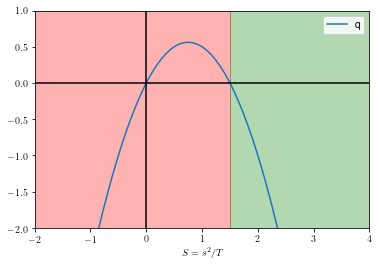
\includegraphics[width=.48\textwidth]{Images/qcas1.png} & 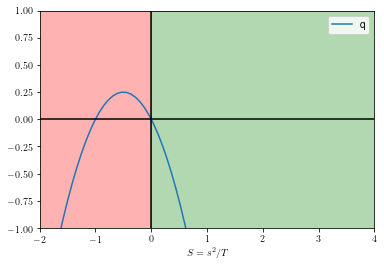
\includegraphics[width=.48\textwidth]{Images/qcas2.png} \\
\end{tabular}
\\
ii) Deux cas possibles sur la condition $q(S)^2-4\sigma(S)>0$:\\

\begin{tabular}{cc}
Une racine positive. & Trois racines positives. \\
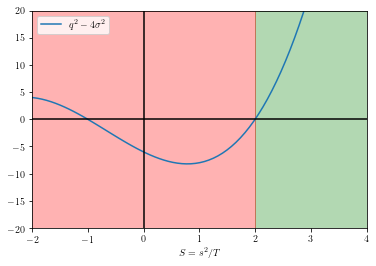
\includegraphics[width=.48\textwidth]{Images/q2cas1.png} & 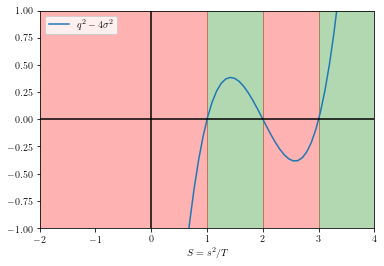
\includegraphics[width=.48\textwidth]{Images/q2cas2.png} \\
\end{tabular}
iii) Deux cas possibles sur la condition $\Delta_A(S) >0$:\\

\begin{tabular}{cc}
Trois racines négatives. & Une racine négative et deux positives.\\
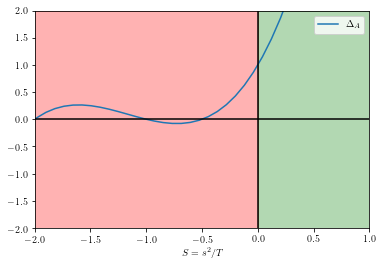
\includegraphics[width=.48\textwidth]{Images/deltacas1.png} & 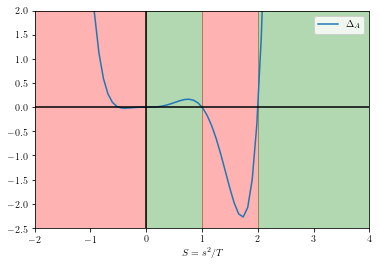
\includegraphics[width=.48\textwidth]{Images/deltacas2.png} \\
\end{tabular}
 \ifdefined\COMPLETE
\else
\end{document}
\fi
